\documentclass{book}

\usepackage[FINAL]{cslipubs}


%%%%%%%%%%%%%%%%%%%%%%%%%%%%%%%%%%%%%%%%%%%%%%
% Beginning of apertium-sme-nob header stuff %
%%%%%%%%%%%%%%%%%%%%%%%%%%%%%%%%%%%%%%%%%%%%%%
% Give us a font that can print \'{a} as á:
\usepackage[T1]{fontenc}
% Let us write á in tex and get á:
\usepackage[utf8]{inputenc} % had some bug with this, but seems to be gone?
\usepackage{graphicx}       % for \includegraphics, only works when {cslipubs} is [FINAL]
\usepackage{amssymb}        % for \square
%%%%%%%%%%%%%%%%%%%%%%%%%%%%%%%%%%%%%%%%
% End of apertium-sme-nob header stuff %
%%%%%%%%%%%%%%%%%%%%%%%%%%%%%%%%%%%%%%%%


\title{A \LaTeX\ Package for CSLI Collections}    % \title{__}  is necessary.
\author{Edie Tor and Ed Itor (eds.)}              % \author{__} is necessary.
\date{May 23, 2002}                               % \date{__}   is optional.


%\raggedbottom   % Uncomment this line if large diagrams cause vertical gaps.

\hfuzz = 2pt

%\crop[]         % Uncomment for centered pages while using [FINAL] option.
%\crop[cam]      % Uncomment for crosshairs that show corners of each page.
%\crop[frame]    % Uncomment for rectangle that shows edges of each page.

\usepackage[comma]{natbib}  % CSLI Pubs favored bibliography package.

\usepackage{chapterbib}     % Allows chapters to have separate bibliographies.
                            % The files example-ch01.tex and example-ch02.tex
                            % contain their own \bibliographystyle{__} and
                            % \bibliography{__} commands.  Run BibTeX
                            % individually on each chapter as follows:
                            %     bibtex example-ch01
                            %     bibtex example-ch02
                            % Do NOT run BibTeX on the main document file.


\usepackage{import}         % Allows chapters to have separate subdirectories.


\usepackage{makeidx}        % Necessary if this book has an Index.
\makeindex                  % Comment out this line when Index is final.


% Some extra macros that CSLI publications sometimes uses.  Not essential.
\usepackage{cslipubs-extra}

% Some more bells and whistles.
%\usepackage{avm}
\usepackage{lingmacros}

% Create your own separate style file and load here to avoid cluttering
% up the preamble more than necessary.  There should be no definitions,
% etc. after the \begin{document} command.
%\usepackage{mymacros}


% The \includeonly{__} command is very useful for processing subsections
% of the entire document.  Read about it in the LaTeX Manual.
%
%\includeonly{example-ch00,example-ch01}


\begin{document}

\frontmatter      %%%%%% Start with Roman page numbers and unnumbered chapters

\maketitle

\setcounter{page}{5}
\setcounter{tocdepth}{0}  % 0 = chapters only in Contents, 1 = sections also.
%\tableofcontents          % LaTeX at least twice for correct Table of Contents.


\mainmatter

%%%%%%%%%%%%%%%%%%%%%%%%%%%%%%%%%%%%%%%%%
% Beginning of apertium-sme-nob chapter %
%%%%%%%%%%%%%%%%%%%%%%%%%%%%%%%%%%%%%%%%%

% TODO general stuff:
% 
% - Mention other _design_ choices that had to do with
%   assimilation (vs dissemination)?
% - should have examples from transfer too, but we've hit the
%   page limit :/


\newcommand{\href}[2]{{\tt #1}} % put hyperref in preamble? TODO
\newcommand{\sme}{{\tt sme}}
\newcommand{\nob}{{\tt nob}}
\newcommand{\smenob}{\sme$\rightarrow{}$\nob}
\newcommand{\nobsme}{\nob$\rightarrow{}$\sme}


\achapter{Evaluating North S\'{a}mi to Norwegian assimilation RBMT}{Trond Trosterud and Kevin Brubeck Unhammer}

\section{Introduction} % and roadmap
\subsection{Roadmap}  
    % \begin{abstract}
We describe the development and evaluation of a rule-based machine
translation (MT) assimilation system from North S\'{a}mi to Norwegian
Bokm{\aa}l\footnote{Source code available from SVN repository\\
  \href{http://apertium.svn.sourceforge.net/svnroot/apertium/trunk/apertium-sme-nob}{http://apertium.svn.sourceforge.net/svnroot/apertium/trunk/apertium-sme-nob}
  under the GNU General Public License.}, built on a combination of
Free and Open Source Software (FOSS) resources: the Apertium platform
and the Giellatekno HFST lexicon and Constraint Grammar disambiguator.
We detail the integration of these and other resources in the system
along with the construction of the lexical and structural transfer,
and evaluate the translation quality using various methods, focusing
on evaluating the users' \textit{comprehension} of the text. Finally,
some future work is suggested.
% Linda: the abstract sounds a bit boring, we do this, then that, 
% then this.. maybe you can put an exciting first sentence including 
% 000the special thing about the work
    % \end{abstract}

We begin with an introduction to the languages and the technology
used, followed by a description of how the system was developed. Then
we evaluate the system with respect to \textit{assimilation}: MT with
the purpose of letting users understand, or get the gist of, a text
written in a language foreign to them (as opposed to
\textit{dissemination}, where the purpose is MT for post-editing).
Finally, we discuss the results and ideas for improvements.


\subsection{The Languages}
North S\'{a}mi (\sme{}) is a Finno-Ugric language spoken by between 
15,000 and 25,000 people in the northern parts of Norway, Sweden and
Finland. Norwegian Bokm{\aa}l (\nob{}) is a North Germanic language
with about 4.5 million speakers, mostly in Norway. North S\'{a}mi %mostly in Norway and where else?
is a highly inflected, agglutinative language, whereas Norwegian
morphology is comparatively simple.

Most \sme{} speakers in Norway understand \nob{}, while most \nob{}
speakers do not understand \sme{}. The languages are completely
unrelated, and the linguistic distance is great, making it hard to
achieve high quality MT results. For a \nobsme{} system to be widely
useful, the quality would have to be good enough that it could be used
for text production (post-editing). On the other hand, a \smenob{}
gisting-quality system (ie. assimilation system) can be useful for the
large group of \nob{} speakers who do not understand \sme{}. Thus we
chose to focus on the \smenob{} direction first.

We do not know of other machine translation (MT) systems between \sme{}
and any Indo-European language, although \citet{tyers2009dpm} describe %Linda: thanks for the citation ;)
a prototype system between North S\'{a}mi and Lule S\'{a}mi.



\section{Design}
 \label{sec:design}

\subsection{The Apertium Pipeline}
This language pair is based on the Apertium MT
platform \citep{forcada2011afp,zubizarreta2009amt}. Apertium provides a
highly modular, shallow-transfer pipeline MT engine, as well as data
for language pairs. Both the engine and the data for all language
pairs (about 30 released pairs as of now) are licensed under the
GPL.\footnote{\href{http://www.fsf.org/licensing/licenses/gpl.html}{http://www.fsf.org/licensing/licenses/gpl.html}}

Apertium language pairs are set up as Unix pipelines, where the
typical pipeline consists of:

\begin{itemize}
\item deformatting (hiding formatting/markup from the engine),
\item source-language (SL) morphological analysis with a finite state
  transducer (FST),
\item disambiguation using a Hidden Markov Model (HMM) and/or
  Constraint Grammar (CG), 
\item lexical transfer (word-translation on the disambiguated source),
\item one or more levels of finite-state based structural transfer
  (reordering, and changes to morphological features),
\item target-language (TL) generation with an FST
\item reformatting (letting format information be shown again)
\end{itemize}

See Figure \ref{fig:modules} below for an overview of the modules used
in this particular language pair. Most Apertium language pairs use the
Apertium lttoolbox FST package for analysis and generation. The
lttoolbox dictionaries are written in XML, where one dictionary may be
compiled both to an analyser and a generator. The \smenob{} pair uses
lttoolbox for \nob{} generation and the translation dictionary, while
the \sme{} analyser is written in the Xerox lexc/twol
formats~\citep{beesley2003fsm}; the reason for this is explained in
Section~\ref{sec:hfst}. Both systems allow generalising over classes
using paradigms/continuation lexicons, but differ in other features.
We use the FOSS package Helsinki Finite State Tools, HFST
\citep{linden2011hfst}\footnote{\href{http://www.ling.helsinki.fi/kieliteknologia/tutkimus/hfst/}{http://www.ling.helsinki.fi/kieliteknologia/tutkimus/hfst/}}
to compile and run the analyser (see Section~\ref{sec:hfst}).

The morphological analysis gives us ambiguous output with no syntactic
information. For morphological (e.g.~part-of-speech) disambiguation,
syntactic annotation/disambiguation and lexical
selection\footnote{Like Word Sense Disambiguation, but restricted to
  senses that have differing translations.}, we use Constraint Grammar
\citep{karlsson1990cgf}\footnote{Using the FOSS package {\tt \small
    VISL CG-3},
  \href{http://beta.visl.sdu.dk/cg3.html}{http://beta.visl.sdu.dk/cg3.html}}.
Morphological disambiguation and syntax are run as one CG module, the
output of which is unambiguous both morphologically (one analysis per
form) and syntactically (each form/analysis is annotated with exactly
one syntactic tag, e.g. \texttt{<@SUBJ>}).

The first CG module\footnote{If the disambiguation rules leaves any
  ambiguity, that CG only prints the first analysis. We may later
  train an HMM to get rid of leftover ambiguity, this would go between
  the two CG modules.} is directly followed by a lexical selection CG
module, which may add subscripts to lemmas in certain contexts in
order to select a different lexical translation.

To make this more concrete, the morphological analysis of the
sentence \textit{Mus lea biebmu vuoššat} ``I have food to boil'' is\\
\texttt{\small \^{}Mus/mun<Pron><Pers><Sg1><Loc>\${}
  \^{}lea/leat<V><IV><Ind><Prs><Sg3>\${}
  \^{}biebmu/biebmat<V><TV><Imprt><Du1>/biebmu<N><Sg><Nom>\${}\\
  \^{}vuoššat/vuoššat<V><TV><Ind><Prs><Pl1>/vuoššat<V><TV><Ind><Prs><Sg2>
  /vuoššat<V><TV><Inf>\${}}, read as \texttt{\small
  \^{}form/lemma1<tags1>/lemma2<tags2>\${}}. The disambiguator removes
the imperative ``feed'' reading of \textit{biebmu} ``food'' by i.a.
checking for the lack of left-hand clause boundaries or conjunctions.
The finite readings of \textit{vuoššat} ``boil'' are removed since
there is a left-hand nominal with an unambiguous finite verb to its
left. Then the readings have syntactic tags appended, e.g.
\textit{vuoššat} gets \texttt{<@$\leftarrow$ADVL>} since it's an
infinitive with a non-abstract nominative to the right.\footnote{The
  actual rules have several other context conditions.} Then the
lexical selection module runs, the only change it makes is adding a
subscript \texttt{:1} to \textit{leat} ``have/be'' in order to select
the ``have'' reading. Its output is \texttt{\small
  \^{}Mun<Pron><Pers><Sg1><Loc><@HAB>\${}
  \^{}leat:1<V><IV><Ind><Prs><Sg3><@+FMAINV>\${}
  \^{}biebmu<N><Sg><Nom><@$\leftarrow{}$SPRED>\${}
  \^{}vuoššat<V><TV><Inf><@$\leftarrow{}$ADVL>\${}}.

% The rest of the output, not enough space for it:
% {\small
% \texttt{\^{}Pron<SN><@HAB><p1><mf><sg><nom>{\^{}jeg<prn><p1><mf><sg><nom>\${}}\${} \^{}verb<SV><@+FMAINV><Ind><pres><p3><sg><impers><NC>{\^{}ha<vblex><pres>\${}}\${} \^{}nom<SN><@$\leftarrow{}$SPRED><ind><m><sg><nom><unc>{\^{}mat<n><m><sg><3>\${}}\${} \^{}verb<SV><@$\leftarrow{}$ADVL><inf><pers><NC>{\^{}koke<vblex><inf>\${}}\${}}\\
% \texttt{\^{}Pron<SN><@HAB><p1><mf><sg><nom>{\^{}jeg<prn><p1><mf><sg><nom>\${}}\${} \^{}verb<SV><@+FMAINV><Ind><pres><p3><sg><impers><NC>{\^{}ha<vblex><pres>\${}}\${} \^{}nom<SN><@$\leftarrow{}$SPRED><ind><m><sg><nom><unc>{\^{}mat<n><m><sg><3>\${}}\${} \^{}verb<SV><@$\leftarrow{}$ADVL><inf><pers><NC>{\^{}koke<vblex><inf>\${}}\${}}\\
% \texttt{\^{}Pron<SN><@HAB><p1><mf><sg><nom>{\^{}jeg<prn><p1><mf><sg><nom>\${}}\${} \^{}verb<SV><@+FMAINV><Ind><pres><p3><sg><impers><NC>{\^{}ha<vblex><pres>\${}}\${} \^{}nom<SN><@$\leftarrow{}$SPRED><ind><m><sg><nom><unc>{\^{}mat<n><m><sg><3>\${}}\${} \^{}verb<SV><@$\leftarrow{}$ADVL><inf><pers><NC>{\^{}koke<vblex><inf>\${}}\${}}\\
% \texttt{\^{}Jeg<prn><p1><mf><sg><nom>\${} \^{}ha<vblex><pres>\${} \^{}mat<n><m><sg><ind>\${} \^{}å<part>\${} \^{}koke<vblex><inf>\${}}\\
% Jeg har mat å koke
% }

Lexical selection is followed by pretransfer (minor format changes in
preparation of transfer) and then a four-stage chunking transfer. The
first stage module first handles lexical transfer using the
translation dictionary, and then performs chunking\footnote{Newer
  Apertium language pairs have lexical transfer as a separate module
  before chunking. This is the plan for \smenob{} too, as it would
  allow matching on both SL and TL patterns, but the possibility was
  only recently added to the transfer engine.} based on patterns of
morphological and syntactic tags (more on structural transfer in
Section \ref{sec:structural-transfer}).

Output from the last transfer module is fed to morphological
generation with the lttoolbox-based \nob{} generator.
% de/reformatters have been mentioned above

\begin{figure*}[htbp]
\begin{center}
 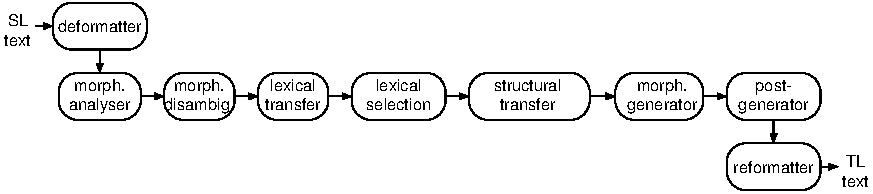
\includegraphics[width=1.0\textwidth]{architecture}
\end{center}
\caption{The Apertium pipeline architecture for \smenob.}
\label{fig:modules}
%\vspace{-1em}
\end{figure*}


\subsection{HFST}
\label{sec:hfst}
One novel feature of apertium-sme-nob is the HFST-based analyser. HFST
makes it possible to compile lexicons and morphologies originally
written for the closed-source Xerox Finite State Tools using FOSS
tools, and run them with Apertium-compatible output formats
\citep{pirinen2011compiling}. As with most Xerox-based analysers, the
\sme{} lexicon and morphology are written in \textbf{lexc} and
compiled into an FST, onto which \textbf{twol} rules are composed
which define the morphophonology. HFST analysers are slower at
compiling and processing than lttoolbox, but certain morphological
phenomena, especially non-concatenative phenomena (e.g. \sme{}
consonant gradation) are impossible---or at least very difficult---to
describe in lttoolbox. Since North S\'{a}mi is quite morphologically
complex, a pure lttoolbox analyser would be hard to maintain.


\section{Development}
  \label{sec:development}

This section describes how the language pair was developed.
\subsection{Resources}
We re-used several FOSS resources in creating this language pair. The
\nob{} generator came from {\tt apertium-nn-nb}
\citep{unhammer2009rfr}, while most of the \sme{} resources came from
the Divvun and Giellatekno S\'{a}mi language technology
projects\footnote{See \href{http://divvun.no}{http://divvun.no} and
  \href{http://giellatekno.uit.no}{http://giellatekno.uit.no}.},
including the lexicon/morphology and disambiguator/syntax CG. Although
we altered our copies from the originals, we continually merged in the
changes that were made in the ``upstream'' versions (ie. the ones
maintaned by Divvun/Giellatekno).

The lexical selection CG and the transfer rules were written from
scratch. The translational dictionary was originally based on various
word-lists from Giellatekno but expanded throughout development.

\subsection{Analysis and derivational morphology}
The morphological analyser was not originally made for machine
translation, and we made several modifications, from minor tag format
changes, to restricting derivational morphology and removing root
forms without translations. Our modifications are all done
automatically using scripts, letting us easily keep the analyser
up-to-date with the upstream version.

The upstream analyser contains many lemmas and readings that are not
in our translation dictionary. These often lead to transfer errors
that can affect the surrounding context, and can suppress the choice
of forms that do have translations. As an example of the latter, the
form \textit{vuovdi} (\textbf{salesperson}) gets a reading both as the
underived noun, and as a derivation of the verb \textit{vuovdit}
(\textbf{to sell}); if both were in the analyser, but only the verb
were in the translation dictionary, the disambiguator might still
choose the noun, and we would end up with an untranslated word where
we could have had a translation. Transfer errors in surrounding
context occur with untrimmed analysers since the translation
dictionary is also used to translate morphological features; e.g. the
\nob{} noun gender is necessarily specified per entry in the
translation dictionary, and the transfer rules may insert
gender-agreeing determiners based on the tags output from the
translation dictionary. Writing heuristic exceptions for every
possible tag omission would be more work than simply adding more good
translations to the dictionary.

We ``trim'' the analyser down to those forms which are in the
translation dictionary. To do this, we use a script which analyses the
lexc source files with the translation dictionary, and outputs only
those entries which have translation analyses.\footnote{The untrimmed
  source files weigh in at about 3.5 MB, trimming this down to 2.6 MB
  is done by a script in our public repository which runs in $<10$
  seconds, and is general enough that other lexc-based language pairs
  can easily use it.}

The original analyser defines quite a lot of rules for derivational
processes. Derivational morphology expands the coverage of the
analyser without having to add new root forms (lexicalisation), but
also makes transfer much harder to deal with, as well as often giving
very odd-sounding translations.
To give an example of the latter, `geafivuohta' is an
adjective$\rightarrow{}$noun derivation of `geafi', meaning `poor'.
Simply carrying over the information that this is an
adjective$\rightarrow{}$noun derivation into the target language
dictionary (if that dictionary also defined derivational processes)
could give us forms that sound like `poorness' or `poority' or
`poordom', whereas giving `geafivuohta' status as a real lexicalised
root form would let us specify that `geafivuohta' should translate to
`poverty'. If we did not use derivations, `geafivuohta' would either
be lexicalised and translated to `poverty', or not translated at all.

Derivations also create extra transfer complexity. A causative verb
derivation requires transfer rules that turn the causative verb into a
periphrastic construction (e.g. `let NP VERB'). If a derivation
changes the part-of-speech from verb to noun, we have to translate the
derivation into a certain verb form that looks right in a noun context
(e.g.~present tense of \nob{} verbs will most of the time look like an
actor noun).\footnote{The alternative would be to define, for each
  \sme{} verb, both a noun and a verb translation on the \nob{} side
  of the translation dictionary, but this takes away the whole point
  of increasing coverage without adding all the root forms.} To make
this even more complex, even a lexicalised form might require a
part-of-speech change in the translation dictionary if there is no
word with the same meaning and part-of-speech in the target language.
The most natural translation to \nob{} of the verb
\textit{muittohuvvat} (``become forgetful'') would be to an auxiliary
+ adjective, \textit{bli glemsk}, and this is what the translational
dictionary specifies. But \textit{muittohuvvat} is not a dynamically
formed derivation, it has a regular entry in the analyser, so we can
also form derivations of it. This means that we also have to ensure
that transfer works for all possible derivations that the analyser can
make, combined with all possible part-of-speech changes specified in
the translational dictionary.

However, since \smenob{} is meant for gisting, where an odd-sounding
translation is more useful than an untranslated word, and resources
for automatically expanding the translation dictionary are scarce, we
decided to allow a restricted set of derivations. We define legal
derivations by the use of additional twol rules which simply forbid
analyses containing certain tags or tag sequences. These twol rules
are composed onto the main analyser in Apertium, but not used
upstream.

\subsection{Disambiguation}
The CG created by Giellatekno was usable in Apertium with only minor
changes to tag naming, requiring very little manual intervention to
keep up-to-date. However, we did add Apertium-only rules which remove
derivations and compound readings if there are lexicalised readings
available, since we want lexically specified translations to override
the guesswork done by derivation transfer. Certain discrepancies in
the tag set of the analyser still exist though, which may affect
disambiguation quality.

\subsection{Lexical selection}
A lexical selection CG was created in order to select between
different possible translations that otherwise share the same
part-of-speech information. Currently it has only 102 rules covering
52 lemmas, mostly high-frequency ones (although 750 other lemmas of
the translation dictionary have at least one alternative translation,
and are awaiting rules). This CG particularly depends on valency and
semantic sets,\footnote{The sets themselves were originally developed
  by Giellatekno for use in the disambiguator.} e.g.
\textit{luohkk\'{a}} by default translates into \textit{bakke},
``hill'', but if we see a context word related to the
\textsc{education} set, we translate into \textit{klasse}, ``(school)
class''.

%Linda: that's a bit short

\subsection{Lexical transfer}
The open classes of the translation dictionary were initiated with
entries from the 9900 lemma dictionary Vuostta\v{s}
Digis\'{a}nit,\footnote{GPL and CC, see
  \href{http://giellatekno.uit.no/words/dicts/index.eng.html}{http://giellatekno.uit.no/words/dicts/index.eng.html}.}
although many ``explanatory'' multiword translations had to be removed
or simplified\footnote{The word \textit{madda} might be translated as
  ``branching part of deer's antlers'' in a human-readable dictionary,
  but in an MT dictionary it has obvious problems -- it sounds
  over-specific and is difficult to wedge into all possible
  grammatical contexts.}. Later on, entries were mostly added
manually. Not including lexical selection alternatives, there are
currently about 3300 verbs, 1400 adjectives and 14000 common nouns in
the translation dictionary.

Unlike with most Apertium language pairs, we did not make an attempt
to change the tag set in the analyser to conform with the Apertium
standard (apart from minor format differences). The change from e.g.
\texttt{<N><Prop>} (proper noun) to \texttt{<np>} or \texttt{<Sg1>} to
\texttt{<sg><p1>} happens in the translation dictionary, mostly using a
\textbf{paradigm} definition to generalise over changes for each part
of speech. Part of the derivation handling also happens here, e.g. 
most passive derivations turn into plain passive forms, while verbs
derived into actor-nouns are transferred to present tense verbs.

We also add special tags used only as a signal to structural transfer,
which are removed before generation. The causative derivation of a
word gets a tag which signals structural transfer to create a
periphrastic `let'-construction, but we also add the same tag to all
forms if the root itself is a lexicalised causative. E.g.
\textit{čálihit} ``let write'' is a lexicalised causative with the
lemma \textit{čállit}; since it is lexicalised, the infinitive is
simply tagged \texttt{<V><TV><Inf>}; since there's no good lexicalised
translation to \nob{}, we translate this lemma (and thus all its
forms) to \textit{skrive} ``write'' along with the tag \texttt{<caus>}
in the translational dictionary. Structural transfer removes
\texttt{<caus>} and outputs \textit{la} ``let'' (putting the main verb
after the causee), and the \nob{} generator never sees any
\texttt{<caus>} tag. If \textit{čálihit} were analysed as a dynamic
derivation of \textit{čállit} ``write'', the lemma would be
\textit{čállit}, while the tag sequence would be
\texttt{<V><TV><Der\_h><V><TV><Inf>} (the ``h-derivation''
\texttt{<Der\_h>} is a causative derivation). In that case we wouldn't
mark the lemma (ie. all forms) with \texttt{<caus>}, but a
\textbf{paradigm} for tag translation would add \texttt{<caus>} only
if the tag sequence contained \texttt{<Der\_h>}.

Verbs are also tagged in the translational dictionary according to the
most likely animacy of the agent\footnote{Currently just manual
  tagging, a corpus-based method should be possible with the use of
  semantic CG sets like HUMAN.} as a signal to structural transfer;
\sme{} often omits subject pronouns (\textbf{pro-drop}), so when
translating to \nob{} and inserting a pronoun we need to know whether
the inserted pronoun should be animate or not.

\subsection{Structural transfer}
\label{sec:structural-transfer}
Our structural transfer is divided into four stages, with different
responsibilities:

\begin{enumerate}

\item Chunking, 63 rules: noun phrases turn into larger chunks,
  prepositions are output based on case information, verb auxiliaries
  and adverbs are output based on verb modality, voice and derivation
  tags.

\item Interchunk 1, 26 rules: simple anaphora resolution (based on
  most recent subject gender), merging coordinated noun phrase chunks,
  moving postpositions before noun phrases.

\item Interchunk 2, 39 rules: major word order changes, inserting
  dropped pronouns, inserting adverbs to indicate verb modality,
  correcting noun phrase definiteness using verb information (e.g.
  subjects of duals are definite).

\item Postchunk, 29 rules: inserting articles/determiners and the
  infinitive marker, tag cleanup in preparation of generation.
\end{enumerate}

Wherever generalisations are possible, we use \textbf{macros} (e.g.
for tranferring agreement information), so rules tend to be fairly
short. A lot of work went into structural transfer compared to what is
typical of Apertium language pairs between more related languages;
e.g. the translator for the closely-related pair
Bokmål$\rightarrow{}$Nynorsk \citep{unhammer2009rfr}, is quite mature
and achieves post-edit quality translations with 2745 lines of
structural transfer code and 107 lines of tag transfer paradigms,
whereas the corresponding numbers for \smenob{} are 9556 and
1002\footnote{Lines of code of course does not correspond one-to-one
  with amount of work, but since the same people did the bulk of the
  work, the numbers should be fairly comparable with each other. All
  numbers are from SVN revision 38590.}.
% TODO: "and numbers from other pairs are also around blah"

\subsection{Generation}
The generator was re-used from the language pair
\texttt{apertium-nn-nb} with very few changes: We added some root
forms to the lexicon, and added a tag to distinguish synthetic from analytic
adjectives (a change which might later be useful in improving
\texttt{apertium-nn-nb}).

\section{Evaluation}
\label{sec:eval}
The na\"{i}ve coverage\footnote{A form is counted as covered if it
  gets at least one analysis. It might have ambiguity which the
  analyser does not cover, thus `na\"{i}ve'.} of the analyser is shown
in Table \ref{table:cov} for legal text (laws), the \sme{} Wikipedia
(wiki) and a corpus of \sme{} news articles. All forms that pass
through the analyser, will also pass through the translation
dictionary, transfer rules and generator, so this shows the coverage
of the other dictionaries (in the \smenob{} direction) as well. Since
derivations are not specified in the translation dictionary, we show
coverage with and without derivation-only analyses counted. The table
also shows the ambiguity rate (amount of analyses per known word) with
and without derivations counted.\footnote{Currently, the ambiguity
  rate is reduced to about 1.04 by the CG disambiguator; in actual
  translations we set the module to simply choose the first analysis
  when there is remaining ambiguity.}


The Wikipedia corpus seems to have very low coverage, but looking over
the unknown words, it seems that many of them are in Finnish, English
or Norwegian (the rest are mostly proper names). The S\'{a}mi Wikipedia
is also written by non-natives, 12.5\% of its words are not recognised
even by Giellatekno's non-normative analyser, as opposed to only 3.5 \% for
a larger, 6.1m reference corpus. The lower coverage for Wikipedia is thus to
be expected.


\begin{table}
  \begin{center}
  \begin{tabular}{crrrrr}
   Corpus     & tokens   & coverage & ambig.      & coverage   & ambig.rate  \\
              &          &          & rate        & w/o deriv  & w/o deriv \\
   laws       &  51706   & 94.68\%  & 2.65        & 86.02\%    & 2.32 \\
   wiki       & 19942    & 77.52\%  & 2.36        & 74.56\%    & 2.19 \\
   news       & 1020250  & 94.72\%  & 2.59        & 90.96\%    & 2.34 \\
  \end{tabular}
    \caption{Na\"{i}ve coverage on several corpora.}
    \label{table:cov}
  \end{center}
\end{table}
In the rest of this section we evaluate the practical performance of
the system using several methods. First we do a word-error rate test,
which shows how well the system would perform in a
post-editing/dissemination setting, then a set of tests meant to find
out how well the system performs in a gisting/assimilation setting.
All tests were run on revision 37177 of \texttt{apertium-sme-nob}\footnote{At which point the repository address was\\
  \href{http://apertium.svn.sourceforge.net/svnroot/apertium/staging/apertium-sme-nob}{http://apertium.svn.sourceforge.net/svnroot/apertium/staging/apertium-sme-nob}}.



\subsection{Word Error Rate on Post-Edited text}
\label{sec:WER}
We did a Word Error Rate test on a short children's
story\footnote{\href{https://apertium.svn.sourceforge.net/svnroot/apertium/branches/xupaixkar/rasskaz}{https://apertium.svn.sourceforge.net/svnroot/apertium/branches/xupaixkar/rasskaz}}
and some paragraphs from a history web
page.\footnote{\href{http://skuvla.info/skolehist/siri97-s.htm}{http://skuvla.info/skolehist/siri97-s.htm}}
The results are shown in Table \ref{table:wer}.\footnote{Our post-edits
  are available from our public repository.} The translator obviously
struggles with the more complex formulations in the history text, and
has a long way to go before being useful for post-editing.


\begin{table}
  \begin{center}
  \begin{tabular}{ccrrr}
   Text       & tokens & Unknown & WER  \\
   children's & 415     & 5      & 45.96\% \\
   history    & 435     & 28     & 60.32\%  \\
  \end{tabular}
    \caption{Word error rate on two short texts.}
    \label{table:wer}
  \end{center}
\end{table}


\subsection{Gisting evaluation}
  
In order to evaluate to what extent the system was able to convey the
meaning of the original to human users, we arranged a test containing
3 parts. All the tests were based on sentences from a parallel corpus
of non-fiction, the corpus had not been used during development of the
MT system. None of the test subjects had any knowledge of \sme{}.

The first test, a multiple choice test, presented 10 \sme{} sentences
drawn from the corpus. For each sentence, the test person also got the
MT output, along with 3 alternative hand-written \nob{} paraphrases
(based on the \sme{} sentence set). Only one of the three paraphrases
was paraphrasing that \sme{} sentence correctly (the other two were
written to be similar, but contain factual mistakes), and the subject
had to use the MT output as a guide to pick which paraphrase
corresponded with the original \sme{} sentence. Example (\ex{1}) shows
the test for one of the sentences\footnote{English glosses were of
  course not shown; note that we keep un-/mistranslated terms
  untranslated in the glosses to indicate what the user actually
  saw.}, where the subject could pick one of a., b. or c., the correct
choice being b. Since the other paraphrases were kept as close as
possible to the meaning of the \sme{} sentence, but had changes that
crucially altered the semantics (e.g. removing the negation, changing
the main content word), an incorrect choice should indicate that the
translation was inadequate in providing understanding.

\enumsentence{
  \small
  \texttt{Original:} Muhto eat diehtán maid mii čáliimet (`But we didn't know what we wrote')\\
  \texttt{Translated:} Men vi visst ikke også skrev vi (`But we didn't known also wrote we')\\
  \texttt{Pick the right alternative:}\\
  a. Vi visste hva vi skrev (`We knew what we wrote')\\
  b. Vi visste ikke hva vi skrev (`We didn't know what we wrote')\\
  c. Vi visste ikke hva de skrev (`We didn't know what they wrote')\\
}

The second test was set up as the first, but instead of the 3
alternatives, the test presented an open question to be answered using
the MT as a guide. This we assumed to test understanding as in Test 1,
but with more reliance on the meaning of content words.

\enumsentence{
  \small
  \texttt{Original:} Goappaš riikkain lea nammaduvvon hálddahuslaš gulahallanolmmoš (`There is appointed an administrative contact from both countries')\\
  \texttt{Translated:} Goappaš på rikene er det oppnevnt administrativt forstående hverandre seg mennesket (`Goappaš on the countries there is appointed an administrative understanding eachother self person')\\
  \texttt{Answer the question:} Hvor kommer kontaktpersonene fra? (`Where do the contact persons come from?')
}

For both test sets the paraphrases / questions were prepared on the
basis of the \sme{} sentence, before they were translated by the
system, in order not to be influenced by the translated output.

% TODO Was the original nob reference not used at all in the above two
% tests?


The third test showed a \sme{} source sentence, then the MT output of
that sentence, followed by the reference translation (5-15 words long)
where at least two of the nouns were removed. For each removed noun,
we instead showed a randomised, clickable list consisting of the
originally removed word, along with a random choice of other
nouns\footnote{Nouns were of the same length ($\pm{} 3$ characters),
  pulled from the same 55128 word long legal text, had the same
  morphological features (gender, definiteness, number) and were never
  ambiguous with verbs. This questionnaire generator is available from
  our public repository (subdirectory \texttt{gisting-eval/generated})
  and should be usable with other translators.} and finally a ``none
seem to fit'' choice. The subjects were instructed to click what
seemed to be the removed word, using the MT as a guide. Ten
consecutive sentences from the same piece of text were shown one at a
time. The test should indicate whether the main content/theme (though
perhaps not the truth conditions) are sufficiently well understood;
the MT output might use the same word used in the answer alternatives,
or one quite similar, or the context might be well enough translated
that the correct alternative seems obvious. Example (\ex{1}) below
shows one of the test sentences, where two word choices had to be made
(in this case both key words happened to translate correctly). All
tests were performed using simple HTML forms.

\enumsentence{
  \small
  \texttt{Original:} Finnmárkkuopmodaga áššegirjjit leat almmolaččat almmolašvuođalága njuolggadusaid mielde
  (`The Finnmark Property's case documents are public according to the rules of the Freedom of Information Legislation')\\
  \texttt{Translated:} Finnmárkkuopmodat saksbøker er offentlig med offentlighetslovens regler
  (`Finnmárkkuopmodat case books are public with the Freedom of Information Legislation's rules')\\
  \texttt{Pick the right alternative:} Finnmarkseiendommens saksdokumenter er offentlige etter \\
  \textsc{$\square$domstolene $\square$kommunene $\square$reglene $\square$deltakerne $\square$ressursene $\square$partene $\square$(ingen som passer)}\\
  i\\
  \textsc{$\square$salgsorganisasjonen $\square$offentlighetsloven $\square$distriktsinndelingen $\square$jordskifteretten $\square$undersøkelsesretten $\square$utmarksdomstolen $\square$(ingen som passer)}\\
  (`The Finnmark Property's case documents are public according to the \\
  \textsc{$\square$court $\square$county $\square$rules $\square$participants $\square$resources $\square$parts $\square$(none of the above)}\\
  of the \\
  \textsc{$\square$sales organisation $\square$Freedom of Information Legislation $\square$regional division $\square$land consolidation $\square$examination right $\square$wilderness court}')
}

The results of all tests are shown in Table \ref{eval}.

\begin{table}[htdp]
\caption{Results of gisting evaluation, 3 different tests}
\begin{center}
\begin{tabular}{lccc}
Type & Multiple & Fill-in & Random \\
Result & 77 \% & 41 \% & 75 \% \\
Number of test subjects & 10 & 14  & 10  \\
\end{tabular}
\end{center}
\label{eval}
\end{table}%



The results from the multiple choice and random word tests correlate
with each other, whereas the fill-in test seems much worse. Open
questions don't allow ``correct guesses'', and the fill-in test was
more vulnerable to holes in the MT output. Four of the 10 test
sentences got no or only one correct answers. It seems that what made
these sentences so hard to understand, was that the system failed to
translate the key word in the sentence. Sentence (\ex{1}), with \nob{}
MT output in (\ex{2}), gives an example.

\enumsentence{
  \small
  \longex{6}{6}
  {... Lillemor Isaksen,  & geas  & lei & gymn\'{a}sa,      & measta & ii}     {fidnen & oahpaheaddjibarggu & go     & son  & lei  & s\'{a}megielat}
  {... Lillemor Isaksen,  & who   & had & secondary.school, & almost & did.not}{get    & teacher.work       & since  & she  & was  & \textbf{saami-speaking}}
  {`... Lillemor Isaksen, who had secondary school, almost did\\
    not get any work as a teacher, since she was \textbf{saami-speaking}'}
}
\enumsentence{
  \small
  \longex{6}{7}
  {... Lillemor Isaksen,  & som  & hadde  & $*$gymn\'{a}sa,  & nesten  & ikke}{han  & f{\aa}tt  & l{\ae}rerarbeidet  & da     & han  & var & samisker}
  {... Lillemor Isaksen,  & who  & had    & $*$gymn\'{a}sa,  & almost  & not }{he   & gotten    & the.teacher.work   & since  & he   & was  & \textbf{saamier}}
  {`... Lillemor Isaksen, who had secondary school, almost did he\\
    not get the teacher work, since he was \textbf{a saamier}'}
}
% wp says 'secondary school' is a general term for what's between primary and university, also it makes the gloss fit better than secondary.high.school

The word \textit{samisker} (here most likely to be interpreted as an
agent noun, on a par with \textbf{carpenter}) does not exist, and is
interpreted by 9 of the informants as ``a Saami'', instead of the
correct ``a Saami speaker''.\footnote{Neither interpretation was in
  the analyser (trimmed or not); the analysis given was the plural of
  the language name, and plurals of common-gendered nouns have the
  same suffix as singular agent nouns in \nob{}, while language names
  are ambiguous with nationality names.} Here, the mistranslation of
the key word blocked a proper understanding of the sentence, despite
the rest of the sentence being translated correctly. The loan word
\textit{gymn\'{a}sa} was not recognised (here marked by a star), but
understandable as it is a loan from Norwegian (\textit{gymnas}).



\subsection{Error analysis}

% eg pröver å sjå på strukturen...


% coverage
The na\"{i}ve lexical coverage of the test sentences was good, 96.7\%,
as compared to the coverage measured on our news corpus (91\%). With
an average sentence length of 14.5 words (as in our test set), the
coverage implies one lexical omission in every second sentence. For
some words, our analysis didn't include all likely readings (e.g.
\textit{muhte} should be ambiguous between a subjunction and a verb,
we only had the verb). In other cases, short (but non-compositional)
idioms were treated as compositional individual words. A lot of
anaphora get the wrong gender, but it's hard to tell how badly this
affects comprehension.

For 3 of the 10 fill-in test sentences the key word (the topic of
the question to be addressed) was not translated. This illuminates
the importance of a good lexical coverage: On average, 95\% coverage implies
one error for each sentence. Also, the pivotal word in the discourse
is likely to carry new meaning, but also be new to
the system. 

% grammatikk
Another challenge is the erroneous insertion of pronouns in pro-drop
sentences. This is more of a problem for dissemination than for
assimilation, but in certain cases the superfluous pronouns may break
the causality chain of the sentence, as in (\ex{1}), with \nob{} MT
output in (\ex{2}):

% NB dieđihuvvo requires T1 fontenc
\enumsentence{
  \small
  \longex{5}{5}
  {... die\dj{}ihuvvo  & ahte  & du\v{s}\v{s}e  & sullii         & 1/3}{skuvllageatnegahtton & ohppiin       & bohte  & oahpahussii}
  {... is.informed     & that  & only           & approximately  & 1/3}{school.duty          & with.teacher  & came   & to.class}
  {`... tells us that only about 1/3 of those of school age with a teacher\\ came to class'} % "with a teacher"? er det rett? TODO
}
\enumsentence{
  \small
  \longex{6}{8}
  {... meddeles     & han  & at    & bare  & omtrent        & 1/3}{$*$skuvllageatnegahtton & med   & en  & l{\ae}rer  & kom   & \textbf{de}    & til  & undervisning}
  {... is.informed  & he   & that  & only  & approximately  & 1/3}{$*$skuvllageatnegahtton & with  & a   & teacher    & came  & \textbf{they}  & to   & class}
  {`... is he informed that only about 1/3 skuvllageatnegahtton\\with a teacher they came to class'}
}

% The point here is the meaning ``it was told that only 1/3 came to
% class''.
%I en rapport fra Kautokeino i 1877 opplyses det at bare om lag 1/3 av de skolepliktige i soknet møtte til undervisning .

The subject status of (the untranslated) \textit{1/3
  skuvllageatnegahtton} is blocked by the insertion of $de$
(``they''). Thus, the otherwise probable (and correct) interpretation
(only 1/3 of X came to class) is suddenly less likely to be detected,
and it is missed by 8 of our informants, several of whom interpret the
sentence as describing a situation where the teacher does not show up.

% det eg pröver på er å forstå korfor ting gjekk skeis:
% - manglande ord? .dix ==> her har vi 96.7, det bör vere ein del
% - dårleg grammatikk .tNx
% - feil ordval? .lex


Some grammatical constructions were too complicated for the system, 
like the sentence
\enumsentence{
  \small
  \shortex{8}
{Jos & ii &  lean & vejola\v{s} & v\'{a}hnemiid & lusa &  vuolgit, & de ...}
{if &  not & was &  possible &    to.parents &    to.PO & travel, &  then ... }
{`If it was not possible to travel to the parents, then ...'}
}



The system interpreted this as a 3rd person pro-drop, and translated
as follows:
\enumsentence{
  \small
  \shortex{9}
{Hvis & han & ikke & hadde & til &   de &  mulige &   foreldrene & reiser ,..}
{If   & he  & not  & had   & to.PR & the & possible & parents &    travels, ...}
{`If he had not to the possible parents travels, ...'}
}

but the correct interpretation is one of a formal subject of
what in Norwegian would have been a cleft construction.

In itself, the erroneous translation in (\ex{0}) would probably be
understandable, but as part of an causal if-X-then-Y construction, it
proved too difficult for half of the informants. What is needed here
is thus better handling of the grammatical construction in question.

% Over-specification is a feature, not a bug, for us:
In the WER tests, we see some errors that are due to our translator
over-specifying, e.g. using ``the two'' as a subject for dual verbs
where ``they'' might be more natural. But for a gisting translator,
over-specific translation is a feature, not a bug.

The ambiguity rate after the disambiguation rules have run is quite
low, but on the other hand we get many erroneous readings, especially
for high-frequency function words (e.g. \textit{maid},
\textbf{also/what/that}). It is also obvious that we need more lexical
selection rules; sometimes the translations simply sound non-fluent,
but in other cases the meaning is altered or lost. E.g.
\textit{lohkat} can mean either \textbf{say} (as in ``Go, he said'')
or \textbf{count} (as in ``I counted to three''), picking the wrong
word here severely hurts understanding.

% Maybe just ditch this paragraph:
The more complex the text, the more we see problems relating to
structural transfer; sometimes we simply do not catch large enough NP
chunks (since we only match fixed-length patterns, they turn into two
chunks instead of one).
% Derivations that work fine by themselves can give problems when they form part of complex NP's.


\section{Discussion and outlook}
Currently, the results of the evaluation of the assimilation indicate
that the MT output provides some help for non-S\'{a}mi speakers in
understanding North S\'{a}mi, but as the results of the fill-in sentence
test showed, users miss important points from isolated sentences at
least.

Both transfer rules and lexical selection could be better. There is an
experimental Apertium package \texttt{apertium-lex-tools} that we plan
to use to automatically create more lexical selection rules.
Disambiguation might be improved by training an HMM to run after the
rule-based disambiguator, although the ambiguity rate is already well
reduced by the rules that are in place.\footnote{An HMM after CG would
  not help with the analyses that are erroneously removed, only those
  that are erroneously left ambiguous}

The na\"{i}ve coverage is very good on paper, even disregarding
derivations, but on the other hand, with a system meant for gisting,
one missing word can take away any chance of understanding the
sentence.

\section*{Acknowledgements}
Development was funded by the Norwegian Ministry of Government
Administration, Reform and Church Affairs. Many thanks to Francis
Tyers, Lene Antonsen, Linda Wiechetek, Berit Eskonsipo, and Sjur
Moshagen, who also contributed much to the development of this
language pair.                  % who did I leave out?



\bibliographystyle {cslipubs-natbib}
\bibliography {apertium}
%%%%%%%%%%%%%%%%%%%%%%%%%%%%%%%%%%%
% End of apertium-sme-nob chapter %
%%%%%%%%%%%%%%%%%%%%%%%%%%%%%%%%%%%


\backmatter
\end{document}

